%%% Local Variables:
%%% mode: latex
%%% TeX-master: "../doc"
%%% coding: utf-8
%%% End:
% !TEX TS-program = pdflatexmk
% !TEX encoding = UTF-8 Unicode
% !TEX root = ../doc.tex

This section shows the final results of the project as well as the partial results that were made along the way.

\subsection{Overview PlanProject vs TogglProject}
To display the difference between the plan projects and the corresponding toggl project three different graphs are displayed in the graphs tab. Those three graphs consist of a total overview, a project overview and an overview where the user can set the start and end date for the analysis.
\subsubsection{Total Overview}
This graph shows the total time planned in all plan projects summed up. (See figure \ref{figure9} ) This is compared with the total tracked time as well as a prognosis of how much time will be needed according to the future plan entries. For example if only one project exists and the whole project has a duration of 5 weeks and every week 2 hours are planned the total time will be 10. If the user is now in week 3 and has worked for 5 hours, the tracked time would show 5 and the prediction would show 9 as week 4 and 5 have both 2 hours planned. This data shows that the user is 1 hour behind the plan project and needs to spend one more hour in week 3.
\begin{figure}[H]
	\centering
	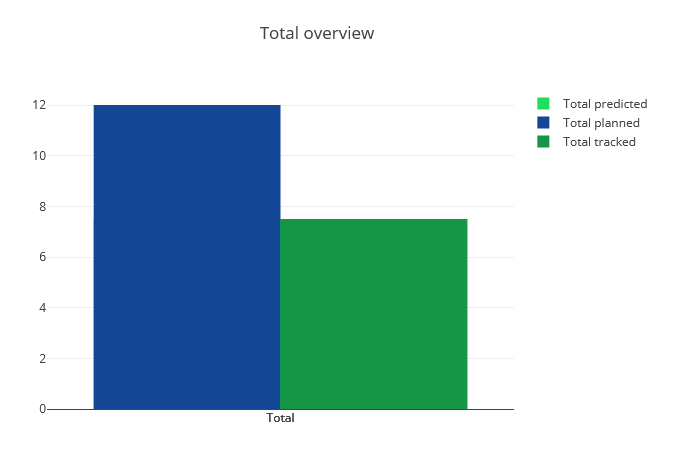
\includegraphics[width=1.0\columnwidth]{TotalOverview}
	\caption{Total Overview}
	\label{figure9}
\end{figure}

\subsubsection{Projects Overview}
This graph is similar to the total overview but the single projects are all show separately. An other minor difference is that the prognosis is added to both the tracked time and the planned time, creating a prediction for both. If there is only one project this overview is mostly the same as the total overview.
\begin{figure}[H]
	\centering
	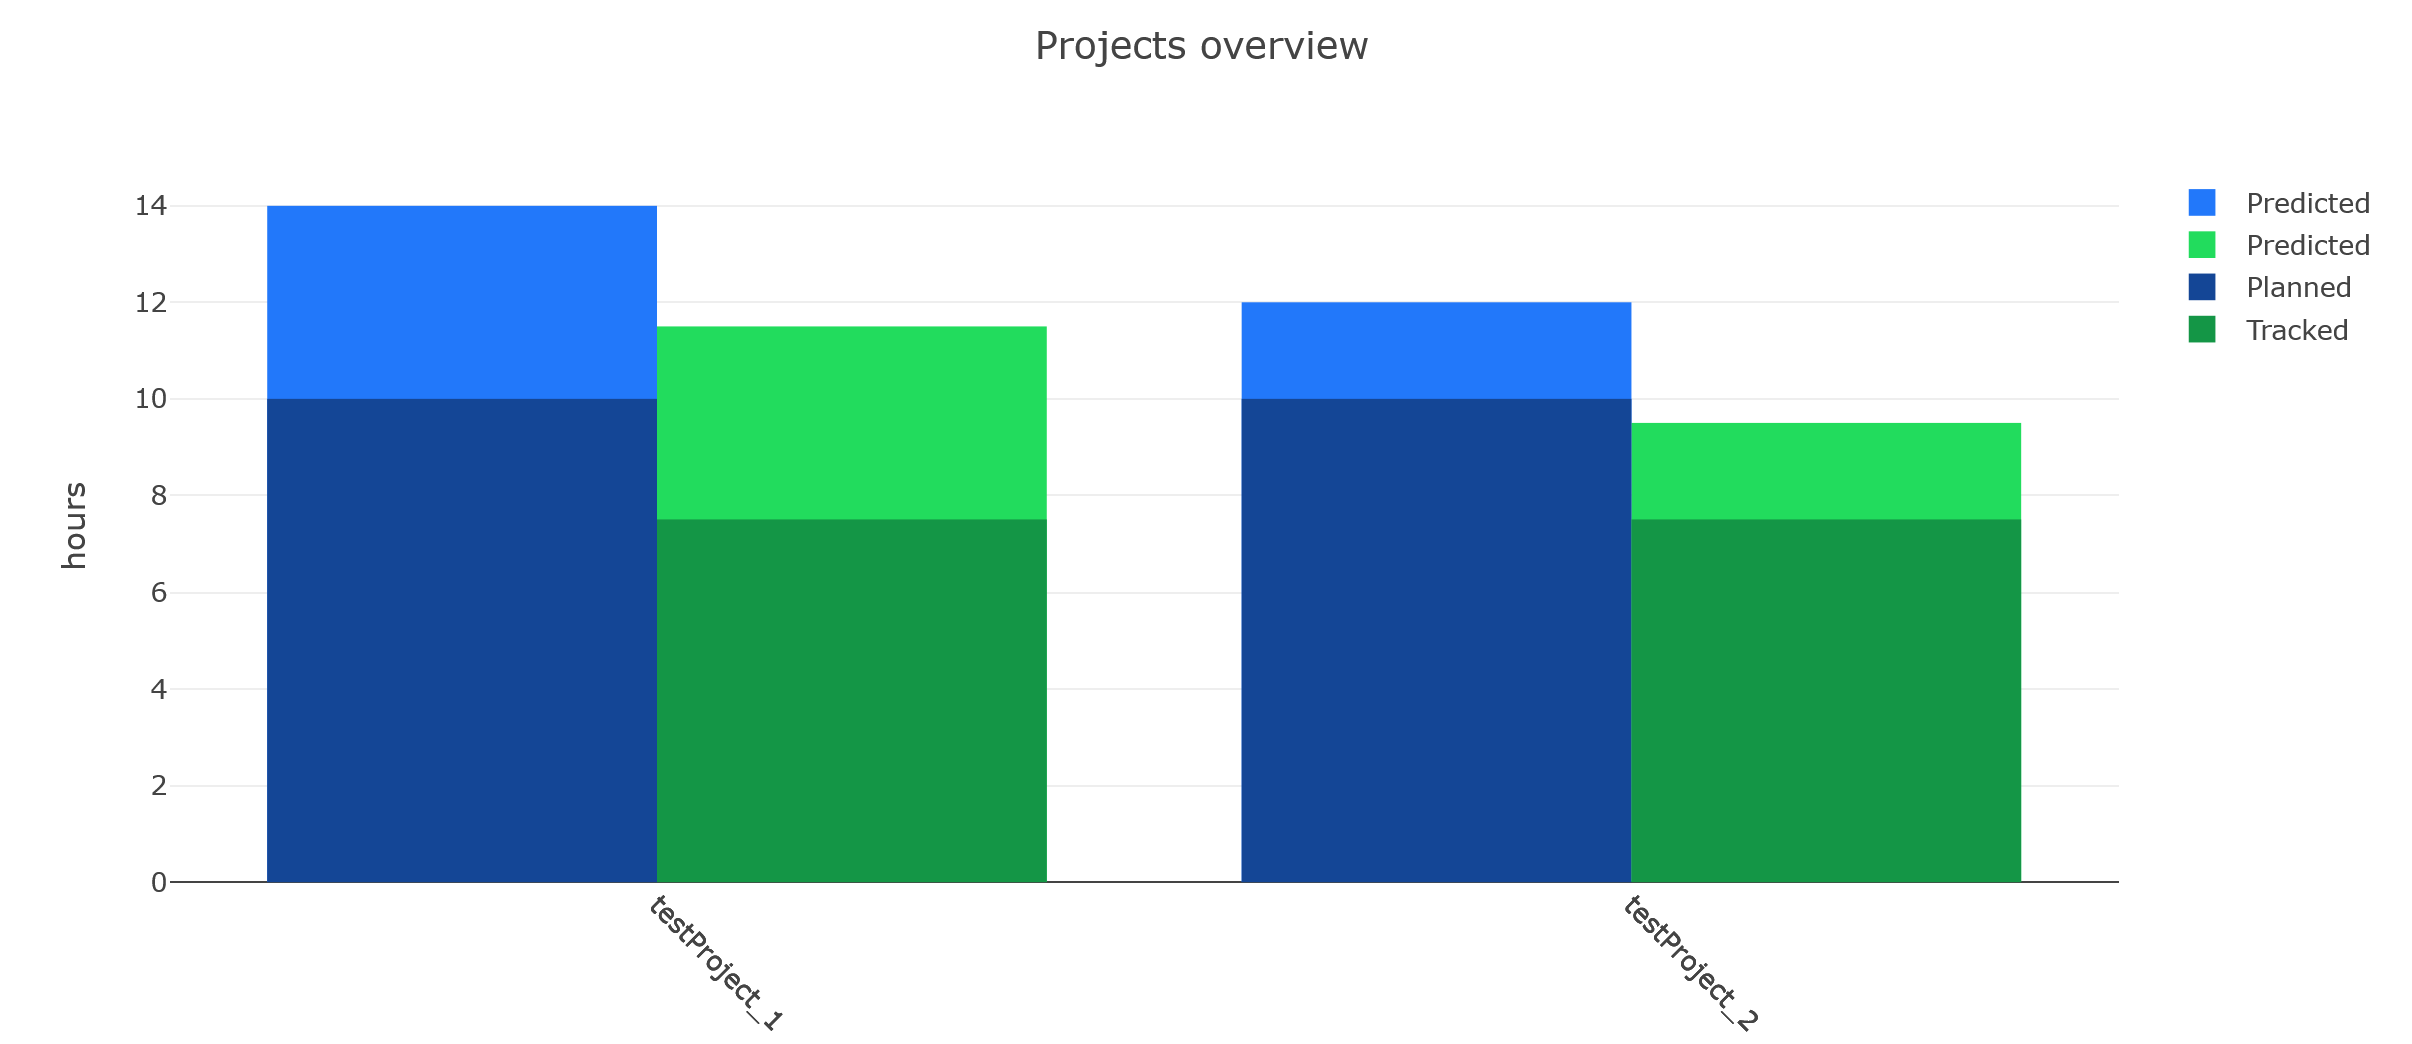
\includegraphics[width=1.0\columnwidth]{ProjectOverview}
	\caption{Total Overview}
	\label{figure10}
\end{figure}

\subsubsection{Project time range overview}
In this graph the user can choose in which time frame the project should be shown. This allows to see if the user is on track and/or if the progression is getting better or worse. As an example if in the first week only half an hour was spent but in the second and third week 3. Then the project overall would show, that half an hour was spent too much and the information of the single weeks would be lost. This graph allows the user to still find these inconsistencies to the planned time.
\begin{figure}[H]
	\centering
	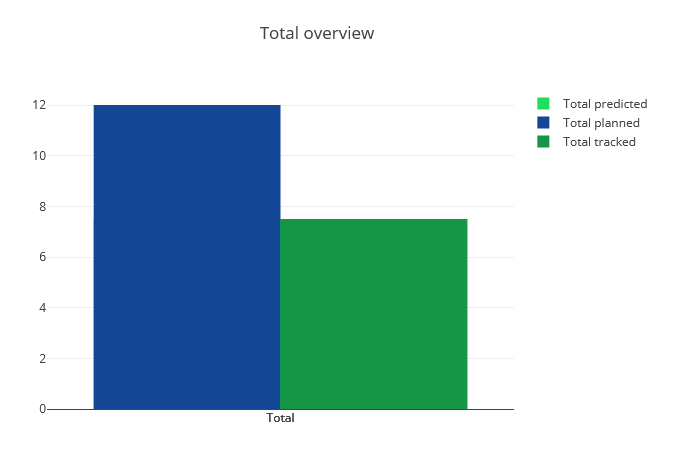
\includegraphics[width=1.0\columnwidth]{TimeOverview}
	\caption{Total Overview}
	\label{figure11}
\end{figure}